% SC4051 --- Chapter 7: Distributed Transactions (0->100)
\chapter{Distributed Transactions: 2PC, 3PC and Spanner}
\label{ch:transactions}

\begin{quote}
\emph{``Transactions are the programmer's way of pretending the world is sequential, even when it is not.''} We make that pretence hold across machines.
\end{quote}

\noindent\fbox{\parbox{\dimexpr\linewidth-2\fboxsep-2\fboxrule}{%
\textbf{From zero: from single-machine ACID to distributed commit.} We start with what ACID means on one disk, then ask how to commit atomically when participants are distributed and may fail. We build 2PC, see why it blocks, fix it partially with 3PC, then leap to Spanner's TrueTime-based external consistency.}}
\vspace{0.4em}

\section*{Learning Outcomes}
After this chapter you will be able to:
\begin{enumerate}[label=(L\arabic*)]
    \item define ACID and explain which letters distribution threatens;
    \item trace two-phase commit (2PC) and identify its blocking window;
    \item describe three-phase commit (3PC) and its extra assumptions;
    \item explain Spanner's TrueTime, commit-wait and externally consistent reads;
    \item compare 2PC/Spanner/Percolator on latency, availability and isolation.
\end{enumerate}

% ============================================================
\section{ACID on One Machine, Then Many}
\label{sec:acid}
On one machine, ACID means: \emph{Atomicity} (all or nothing), \emph{Consistency} (invariants preserved), \emph{Isolation} (concurrent transactions appear serial), \emph{Durability} (committed data survives crashes). The write-ahead log (WAL) plus two-phase locking or MVCC implements this with one disk as the ground truth.

Distribute the data and each letter gets harder. Atomicity now needs \emph{distributed commit}: either all participants commit or all abort, even if some crash mid-protocol. Isolation now spans shards. Durability now means replicated durability. Consistency remains the application's invariant, but the system must not break it.

A \emph{distributed transaction} touches participants $P_1,\dots,P_n$ coordinated by a transaction manager (TM). Each participant can vote to commit or abort; the group must agree.

% ============================================================
\section{Two-Phase Commit (2PC)}
\label{sec:2pc}
2PC is the classic blocking atomic-commit protocol:

\paragraph{Phase 1 (Voting).} TM sends \texttt{PREPARE} to all participants. Each participant that can commit writes a \texttt{PREPARED} record to its WAL and replies \texttt{YES}; otherwise it writes \texttt{ABORT} and replies \texttt{NO}.

\paragraph{Phase 2 (Decision).} If all voted \texttt{YES}, TM writes \texttt{COMMIT} and sends \texttt{COMMIT}; otherwise it writes \texttt{ABORT} and sends \texttt{ABORT}. Participants that receive the decision apply it and ack.

If any participant votes \texttt{NO} or fails to respond, the transaction aborts. The WAL records make crash-recovery possible: on restart a participant in \texttt{PREPARED} state must contact the TM to learn the outcome.

\begin{figure}[h]
\centering
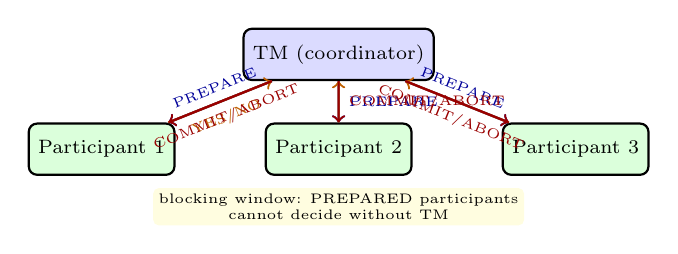
\begin{tikzpicture}[scale=0.86, every node/.style={font=\scriptsize},
  box/.style={draw,rounded corners=3pt,minimum width=1.85cm,minimum height=0.65cm,align=center,thick}]
\node[box,fill=blue!14] (tm) at (3.5,2.6) {TM (coordinator)};
\node[box,fill=green!14] (p1) at (0,1.2) {Participant 1};
\node[box,fill=green!14] (p2) at (3.5,1.2) {Participant 2};
\node[box,fill=green!14] (p3) at (7.0,1.2) {Participant 3};
\draw[->,thick,blue!60!black] (tm) -- (p1) node[midway,above,sloped,font=\tiny] {PREPARE};
\draw[->,thick,blue!60!black] (tm) -- (p2) node[midway,right,font=\tiny] {PREPARE};
\draw[->,thick,blue!60!black] (tm) -- (p3) node[midway,above,sloped,font=\tiny] {PREPARE};
\draw[<-,thick,orange!75!black] (tm) -- (p1) node[midway,below,sloped,font=\tiny] {YES/NO};
\draw[<-,thick,orange!75!black] (tm) -- (p2);
\draw[<-,thick,orange!75!black] (tm) -- (p3);
\draw[->,thick,red!60!black] (tm) -- (p1) node[midway,below,sloped,font=\tiny] {COMMIT/ABORT};
\draw[->,thick,red!60!black] (tm) -- (p2) node[midway,right,font=\tiny] {COMMIT/ABORT};
\draw[->,thick,red!60!black] (tm) -- (p3) node[midway,below,sloped,font=\tiny] {COMMIT/ABORT};
\node[font=\tiny,align=center,fill=yellow!12,rounded corners=2pt,inner sep=2pt] at (3.5,0.35) {blocking window: PREPARED participants\\cannot decide without TM};
\end{tikzpicture}
\caption{Two-phase commit: voting then decision. Participants in PREPARED state are blocked until the TM's decision arrives.}
\label{fig:2pc}
\end{figure}

\paragraph{Blocking.} If the TM crashes after some participant has entered \texttt{PREPARED} but before broadcasting the decision, those participants are \emph{blocked}: they cannot commit (some other participant may have been told to abort) and cannot abort (some may have been told to commit). They must wait for TM recovery. This unavailability is fundamental to 2PC over async networks---it is not a bug but a consequence of needing consensus on the outcome.

\begin{lstlisting}[language=Python]
# 2PC simulation: coordinator + participants with WAL states
class Participant:
    def __init__(self, pid, can_commit=True):
        self.pid, self.can_commit = pid, can_commit
        self.state = "INIT"  # INIT -> PREPARED/ABORTED -> COMMITTED/ABORTED
    def on_prepare(self):
        if self.can_commit:
            self.state = "PREPARED"  # WAL write before reply
            return "YES"
        self.state = "ABORTED"
        return "NO"
    def on_decision(self, decision):
        self.state = decision  # COMMITTED or ABORTED
        return f"P{self.pid}:{self.state}"

class Coordinator:
    def __init__(self, participants):
        self.participants = participants
        self.state = "INIT"
    def commit(self):
        votes = [p.on_prepare() for p in self.participants]
        print("votes:", votes)
        if all(v=="YES" for v in votes):
            self.state = "COMMIT"
        else:
            self.state = "ABORT"
        # Phase 2: broadcast decision
        for p in self.participants:
            if p.state == "PREPARED":
                print(p.on_decision("COMMITTED" if self.state=="COMMIT" else "ABORTED"))
        return self.state

# Happy path
ps = [Participant(i) for i in range(3)]
print("result:", Coordinator(ps).commit())
# One participant votes NO -> abort
ps2 = [Participant(0), Participant(1, can_commit=False), Participant(2)]
print("result:", Coordinator(ps2).commit())
\end{lstlisting}

% ============================================================
\section{Three-Phase Commit (3PC) and Non-Blocking Attempts}
\label{sec:3pc}
3PC adds a \texttt{PRE-COMMIT} phase between voting and commit so that if a participant is in \texttt{PRE-COMMIT}, it knows every other participant voted \texttt{YES}. Then, if the TM fails, participants can run a termination protocol among themselves: if any is in \texttt{COMMIT}, commit; if any is in \texttt{ABORT}, abort; if all are in \texttt{PREPARED}, they need to agree---but with the extra phase the ambiguity window shrinks.

Crucially, 3PC is non-blocking \emph{only} under synchrony assumptions (bounded delay + perfect failure detection). Under asynchrony or partitions it either blocks or risks violating safety---which FLP tells us is unavoidable for deterministic consensus. In practice, systems prefer 2PC + a highly available TM (itself replicated via Paxos/Raft) over 3PC.

\begin{figure}[h]
\centering
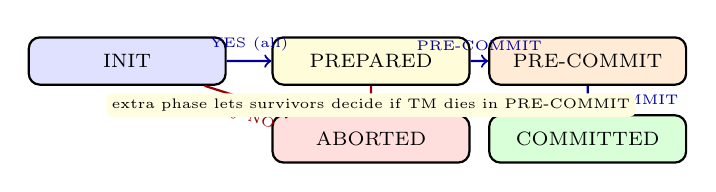
\begin{tikzpicture}[scale=0.86, every node/.style={font=\scriptsize},
  s/.style={draw,rounded corners=4pt,minimum width=2.5cm,minimum height=0.60cm,align=center,thick}]
\node[s,fill=blue!12] (init) at (0,2.0) {INIT};
\node[s,fill=yellow!15] (prep) at (3.6,2.0) {PREPARED};
\node[s,fill=orange!16] (precom) at (6.8,2.0) {PRE-COMMIT};
\node[s,fill=green!15] (com) at (6.8,0.85) {COMMITTED};
\node[s,fill=red!13] (abo) at (3.6,0.85) {ABORTED};
\draw[->,thick,blue!60!black] (init) -- (prep) node[midway,above,font=\tiny] {YES (all)};
\draw[->,thick,blue!60!black] (prep) -- (precom) node[midway,above,font=\tiny] {PRE-COMMIT};
\draw[->,thick,blue!60!black] (precom) -- (com) node[midway,right,font=\tiny] {COMMIT};
\draw[->,thick,red!60!black] (init) -- (abo) node[midway,below,sloped,font=\tiny] {any NO};
\draw[->,thick,red!60!black] (prep) -- (abo) node[midway,right,font=\tiny] {abort};
\node[font=\tiny,fill=yellow!12,rounded corners=2pt,inner sep=2pt] at (3.6,1.35) {extra phase lets survivors decide if TM dies in PRE-COMMIT};
\end{tikzpicture}
\caption{3PC state transitions. The PRE-COMMIT phase makes the protocol non-blocking under synchrony but not under asynchrony.}
\label{fig:3pc}
\end{figure}

% ============================================================
\section{Spanner: TrueTime and Externally Consistent Transactions}
\label{sec:spanner}
Spanner (Corbett et al., 2012) is a globally distributed database that provides \emph{externally consistent} (linearizable) read-write transactions with SQL, using TrueTime and 2PC.

\paragraph{TrueTime.} Each datacenter has GPS and atomic clocks. TrueTime returns an interval $[earliest, latest]$ guaranteed to contain the true absolute time; typical $\epsilon\approx 2$--$7$\,ms. Spanner assigns each transaction a timestamp $ts$ and enforces \emph{commit-wait}: the coordinator waits until $TT.now().earliest > ts$ before making the write visible. This ensures that if transaction $T_1$ commits before $T_2$ starts in real time, $ts(T_1) < ts(T_2)$---so timestamp order respects external order.

\paragraph{Read-write transactions.} Spanner runs 2PC across shards, but the prepare phase also picks a prepare timestamp. The coordinator chooses $ts = \max(prepare\_ts) + \text{epsilon}$ and then commit-waits. Paxos-replicated shards provide durability per group. Read-only transactions pick a timestamp in the past and read the snapshot at that timestamp from the nearest replica---lock-free, fast, and still externally consistent.

\begin{figure}[h]
\centering
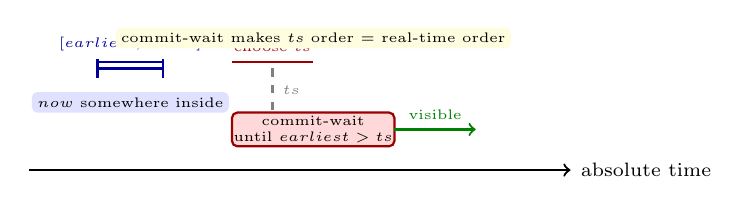
\begin{tikzpicture}[scale=0.86, every node/.style={font=\scriptsize}]
\draw[->,thick] (0,0) -- (8.0,0) node[right] {absolute time};
% TrueTime intervals
\draw[thick,blue!60!black] (1.0,1.6) -- (2.0,1.6) node[midway,above,font=\tiny] {$[earliest, latest]$};
\draw[|-|,blue!60!black,thick] (1.0,1.5) -- (2.0,1.5);
\node[font=\tiny,fill=blue!12,rounded corners=2pt,inner sep=2pt] at (1.5,1.0) {$now$ somewhere inside};
% commit wait
\draw[thick,red!60!black] (3.0,1.6) -- (4.2,1.6) node[midway,above,font=\tiny] {choose $ts$};
\fill[red!15,draw=red!60!black,thick,rounded corners=2pt] (3.0,0.35) rectangle (5.4,0.85);
\node[font=\tiny,align=center] at (4.2,0.60) {commit-wait\\until $earliest>ts$};
\draw[->,thick,green!50!black] (5.4,0.60) -- (6.6,0.60) node[midway,above,font=\tiny] {visible};
\draw[thick,gray,dashed] (3.6,1.5) -- (3.6,0.85) node[midway,right,font=\tiny] {$ts$};
\node[font=\tiny,fill=yellow!12,rounded corners=2pt,inner sep=2pt] at (4.2,1.95) {commit-wait makes $ts$ order = real-time order};
\end{tikzpicture}
\caption{Spanner commit-wait: the coordinator picks $ts$ inside the TrueTime interval and waits until TrueTime guarantees $ts$ is in the past before exposing the write.}
\label{fig:spanner-wait}
\end{figure}

\begin{lstlisting}[language=Python]
# Spanner commit-wait intuition with TrueTime intervals
import random

class TrueTime:
    def __init__(self, epsilon_ms=5):
        self.eps = epsilon_ms
    def now(self, real_ms):
        # return [earliest, latest] containing real time
        return real_ms - self.eps, real_ms + self.eps

tt = TrueTime(epsilon_ms=5)
# Transaction picks ts, then waits until earliest > ts
def commit_with_wait(real_pick_ms):
    earliest, latest = tt.now(real_pick_ms)
    ts = latest  # Spanner picks ts within interval, here worst case latest
    # wait until TrueTime.earliest > ts
    wait_until = ts + tt.eps + 1  # earliest = real - eps > ts  => real > ts+eps
    print(f"pick at real={real_pick_ms} interval=[{earliest},{latest}] ts={ts} -> visible after real>{wait_until}")
    return ts

t1 = commit_with_wait(100)
t2 = commit_with_wait(120)
print(f"external order: T1 before T2, timestamp order: {t1} < {t2} = {t1 < t2}")

# Read-only transaction: pick timestamp in the past, read snapshot -- no locks
def snapshot_read(read_ts, writes):
    # writes: list of (ts, key, value)
    snapshot = {k: v for ts,k,v in writes if ts <= read_ts}
    return snapshot

writes = [(t1,"x",10),(t2,"x",20)]
print("read at t1 sees:", snapshot_read(t1, writes))
print("read at t2 sees:", snapshot_read(t2, writes))
\end{lstlisting}

% ============================================================
\section{Exercises}
\label{sec:ch07-exercises}
\begin{enumerate}[label=E7.\arabic*, leftmargin=*, itemsep=0.6em]
    \item \textbf{2PC blocking.} Construct an execution where the TM crashes after sending \texttt{PREPARE} and one participant has replied \texttt{YES} while another has not yet voted. Show why the \texttt{YES} voter is blocked and what information it would need to unblock without the TM.
    \item \textbf{3PC vs.\ synchrony.} Explain why 3PC's non-blocking guarantee requires a perfect failure detector (synchrony). Give a partition scenario where 3PC would violate safety if it tried to stay non-blocking under asynchrony.
    \item \textbf{Spanner timestamps.} Two transactions $T_1,T_2$ commit with TrueTime $\epsilon=5$\,ms. $T_1$'s commit-wait ends at real time $105$\,ms, $T_2$ starts at $107$\,ms. Prove $ts(T_1)<ts(T_2)$. What breaks if commit-wait is skipped?
    \item \textbf{2PC + Paxos TM.} How does replicating the TM with Paxos/Raft mitigate 2PC's blocking? Describe the recovery path when the old TM leader crashes in \texttt{PREPARED} and the new TM leader takes over. What WAL records does it need?
    \item \textbf{Isolation levels.} Compare Spanner (external consistency), Percolator (snapshot isolation) and 2PC with 2PL (serializable) on (a) read-only latency, (b) write latency, (c) availability under one shard down. Which would you choose for a global ad-auction ledger vs.\ a social feed?
\end{enumerate}

% ============================================================
\section*{Chapter Notes}
Gray (1978) and Lampson--Sturgis (1979) for 2PC; Skeen (1981) for 3PC and its impossibility without synchrony. Spanner: Corbett et al., ``Spanner: Google's globally-distributed database'' (OSDI, 2012); TrueTime details in the same paper. Percolator: Peng--Dabek (OSDI, 2010) for snapshot isolation on Bigtable. For a textbook treatment of commit protocols see Bernstein--Hadzilacos--Goodman, \emph{Concurrency Control and Recovery in Database Systems} (1987) and Kleppmann Ch.~9.

% End of Chapter 7
